% !TeX program = lualatex
% ================================================================
% Polish Tier 3 Vocabulary Version of CalculationsRevision
%
% Generated by the server using the following settings:
%
%   language            Polish (pol)
%   text direction      left to right
%   font                Noto Serif
%   fallback font       Noto Serif
%   built from          latex/worksheets/arithmetic/calculationsRevision.tex
%   vocabulary key      latex/worksheets/arithmetic/calculationsRevision/L2/pol/calculationsRevision_polishKey.tex
%   tier 3 vocabulary   green   RGB 0 128 0
%   English text        black   RGB 0 0 0
%   Polish text         purple  RGB 112 48 160
%   layout macros       version 3
%
% Please don't edit any information in this comment block - the server
% compares it against the current settings and rebuilds this file when
% they differ, so changes here would be overwritten. However, feel free
% to make updates to the LaTeX below if you want to edit it.
% ================================================================

\documentclass[12pt,a4paper]{article}
% ================================================================
% Copied from the English sheet this was translated from, so that
% anything it sets up for itself still works here
% ================================================================
% Packages for formatting
\usepackage[margin=1in]{geometry}
\usepackage{multicol}
\usepackage{amsmath,amssymb}
\usepackage{array}
\usepackage{fancyhdr}
\usepackage{setspace}
\usepackage{tikz}

\pagestyle{fancy}
\fancyhf{}
\lhead{Year 7 Arithmetic Revision}
\rhead{Page \thepage}
\setlength{\parindent}{0pt}
\setstretch{1.2}

% Characters this language's font has not got are borrowed from another,
% rather than being silently dropped - see docs/translated-sheet-latex.md
\directlua{%
  if luaotfload and luaotfload.add_fallback then
    luaotfload.add_fallback("eallatinfallback",
      { "Noto Serif:mode=harf;" })
  else
    tex.error("this luaotfload is too old to register a fallback font")
  end
}
\usepackage[english]{babel}
\babelprovide[import]{polish}
\babelfont[polish]{rm}[Renderer=Harfbuzz, BoldFont={Noto Serif}, ItalicFont={Noto Serif}, BoldItalicFont={Noto Serif}, RawFeature={fallback=eallatinfallback}]{Noto Serif}
\babelfont[polish]{sf}[Renderer=Harfbuzz, BoldFont={Noto Serif}, ItalicFont={Noto Serif}, BoldItalicFont={Noto Serif}, RawFeature={fallback=eallatinfallback}]{Noto Serif}
\newcommand{\ealtext}[1]{\foreignlanguage{polish}{#1}}
\newcommand{\ealtextblock}[1]{{\raggedright\foreignlanguage{polish}{#1}\par}}
% ================================================================
% EAL layout helpers
% ================================================================
\usepackage{xcolor}

\definecolor{ealkeycolour}{RGB}{0,128,0}
\definecolor{ealenglish}{RGB}{0,0,0}
\definecolor{ealtwocolour}{RGB}{112,48,160}

\newsavebox{\ealboxen}
\newsavebox{\ealboxtr}
\newlength{\ealglosswd}
\newlength{\ealglossraise}
\setlength{\ealglossraise}{1.15em}

% a tier 3 word, in English and in translation alike
\newcommand{\ealkey}[1]{\textcolor{ealkeycolour}{#1}}
\newcommand{\ealkeytr}[1]{\textcolor{ealkeycolour}{\ealtext{#1}}}

% One translated word above one English word. Built from kernel
% primitives, never a tabular, which would break wherever the sheet
% loads array, booktabs or tabularx. The box is as wide as the wider of
% the two, so a long translation pushes its neighbours aside instead of
% overlapping them, and it claims its full height so a table row or a
% TikZ node makes room for it.
\newcommand{\ealgloss}[2]{%
  \sbox{\ealboxen}{\ealkey{#1}}%
  \sbox{\ealboxtr}{\small\textcolor{ealtwocolour}{\ealtext{#2}}}%
  \setlength{\ealglosswd}{\wd\ealboxen}%
  \ifdim\wd\ealboxtr>\ealglosswd\setlength{\ealglosswd}{\wd\ealboxtr}\fi
  \leavevmode
  \makebox[\ealglosswd][c]{%
    \makebox[0pt][c]{\usebox{\ealboxen}}%
    \makebox[0pt][c]{\raisebox{\ealglossraise}{\usebox{\ealboxtr}}}%
  }%
}

% opens up line spacing around a block of glosses, so the raised
% translations sit clear of the line above
\newenvironment{ealglossed}{\par\linespread{2.1}\selectfont\ignorespaces}{\par}

% a whole translated sentence above its English counterpart. block level,
% so it does not belong inside a tabular cell
\newcommand{\ealpara}[2]{%
  \par\addvspace{0.5\baselineskip}%
  {\color{ealtwocolour}\ealtextblock{#1}}%
  \penalty200
  {\color{ealenglish}#2\par}%
  \addvspace{0.5\baselineskip}%
}

\begin{document}

\begin{ealglossed}
\begin{center}
    \vspace{2em}
    {\LARGE \textbf{Four \ealgloss{Operations}{działania} Revision Worksheet}} \\[0.5em]
    \vspace{1em}
    \textbf{\ealgloss{Whole Numbers}{liczby całkowite nieujemne}, \ealgloss{Decimals}{ułamki dziesiętne}, and \ealgloss{Negative}{ujemne} Numbers} \\[0.5em]
    \vspace{1em}
 \end{center}
\end{ealglossed}

\hrule
\vspace{1em}

\section*{Section 1: \ealgloss{Addition}{dodawanie} and \ealgloss{Subtraction}{odejmowanie}}

\begin{ealglossed}
\textbf{Remember:} Line up the \ealgloss{decimal points}{przecinki dziesiętne} carefully. When working with \ealgloss{negatives}{ujemne}, think about the \ealgloss{sign}{znak}!
\end{ealglossed}

\begin{multicols}{2}
\begin{enumerate}
    \item $45 + 376 =$
    \vspace{2em}
    \item $328.5 + 19.47 =$
    \vspace{2em}
    \item $7.63 + (-2.8) =$
    \vspace{2em}
    \item $-12 + 7 =$
    \vspace{2em}
    \item $56.3 - 18.72 =$
    \vspace{2em}
    \item $-4 - (-9) =$
\end{enumerate}
\end{multicols}


\section*{Section 2: \ealgloss{Multiplication}{mnożyć}}

\begin{ealglossed}
\textbf{Remember:} 
\begin{itemize}
    \item Count the \ealgloss{signs}{znaki}: an \textbf{\ealgloss{even}{parzysta}} number of \ealgloss{negatives}{ujemne} gives a \ealgloss{positive}{liczba dodatnia} answer, an \textbf{\ealgloss{odd}{liczba nieparzysta}} number gives a \ealgloss{negative}{ujemna} answer.
    \item We need to be careful when multiplying \ealgloss{decimals}{ułamki dziesiętne}, and keep track of the \ealgloss{decimal point}{przecinek dziesiętny}, three methods are described below.
\end{itemize}
\end{ealglossed}


\begin{ealglossed}
For the example \ealgloss{multiplication}{mnożyć}: $3.4 \times 1.2$, the three options are:
\end{ealglossed}

\subsection*{1. Factoring Up to \ealgloss{Whole Numbers}{liczby całkowite nieujemne}}

\begin{ealglossed}
We can make both numbers whole by multiplying by \ealgloss{powers}{potęgi} of 10. These are $10$, $100$, $1\,000$, $10\,000$, \dots \quad etc.
\end{ealglossed}

Multiply \(3.4\) by \(10\) to make it \(34\).  
Multiply \(1.2\) by \(10\) to make it \(12\).

Now we have:
\[
34 \times 12 = 408
\]

But we multiplied the numbers by \(10 \times 10 = 100\),  
so we divide the answer by \(100\):

\[
\frac{408}{100} = 4.08
\]

---

\subsection*{2. Counting \ealgloss{Decimal Places}{miejsca dziesiętne}}

\begin{ealglossed}
\begin{enumerate}
    \item Multiply the numbers as if there are no \ealgloss{decimal points}{przecinki dziesiętne}.  
    \item Count how many \ealgloss{decimal places}{miejsca dziesiętne} there are in total in the question.  
    \item Put that many \ealgloss{decimal places}{miejsca dziesiętne} back into your answer.
\end{enumerate}
\end{ealglossed}

\begin{ealglossed}
\textbf{Example:} \(3.4 \times 1.2\)

Ignore the \ealgloss{decimals}{ułamki dziesiętne}: \(34 \times 12 = 408\)

There is \textbf{1 \ealgloss{decimal place}{miejsce dziesiętne}} in 3.4 and \textbf{1} in 1.2, so \textbf{2 in total.}
\end{ealglossed}

So the answer is \(4.08\) 

---

\subsection*{3. Lattice Method with \ealgloss{Decimal}{ułamek dziesiętny} Alignment}

\begin{ealglossed}
You can use the lattice method to track the \ealgloss{decimal points}{przecinki dziesiętne} too.
\end{ealglossed}

\begin{center}
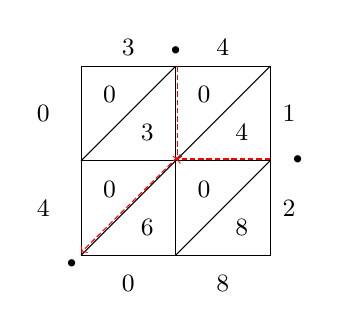
\begin{tikzpicture}[scale=1.2, every node/.style={font=\small}]

% Grid (2x2 for digits 3,4 × 1,2)
\draw (0,0) rectangle (2,2);
\draw (1,0) -- (1,2);
\draw (0,1) -- (2,1);


\draw (0,0) -- (2,2);
\draw (1,0) -- (2,1);
\draw (0,1) -- (1,2);


% Top numbers (3 and 4)
\node at (0.5,2.2) {3};
\node at (1.5,2.2) {4};

% Side numbers (1 and 2)
\node at (2.2,1.5) {1};
\node at (2.2,0.5) {2};

% Products in cells (tens and ones separated)
% 3×1 = 3, 4×1 = 4, 3×2=6, 4×2=8
\node at (0.3,1.7) {0};
\node at (0.7,1.3) {3};

\node at (1.3,1.7) {0};
\node at (1.7,1.3) {4};

\node at (0.3,0.7) {0};
\node at (0.7,0.3) {6};

\node at (1.3,0.7) {0};
\node at (1.7,0.3) {8};

% Diagonal sums
\node at (1.5,-0.3) {8};
\node at (0.5,-0.3) {0};
\node at (-0.4,0.5) {4};
\node at (-0.4,1.5) {0};

% Decimal point placement
\node at (2.3,1) {\Huge$\cdot$};
\node at (1, 2.15) {\Huge$\cdot$};

% decimal point movement to result

\draw[red, dash pattern=on 2pt off 1pt, ->] (1.02,2.0) -- (1.02,1);
\draw[red, dash pattern=on 2pt off 1pt, ->] (2,1.02) -- (1,1.02);
\draw[red, dash pattern=on 2pt off 1pt, ->] (1.02,1.04) -- (0,0.03);

\node at (-0.1,-0.1) {\Huge$\cdot$};

\end{tikzpicture}

\end{center}


\begin{ealglossed}
Find where the \ealgloss{decimal points}{przecinki dziesiętne} in each number meet, then follow the diagonal down to the left, that will be where the \ealgloss{decimal point}{przecinek dziesiętny} is in the answer.
\end{ealglossed}

\vspace{1em}

In the example above we get \(4.08\), the same as before!

---

\vspace{2em}

Now try these questions:

\begin{center}
\begin{tabular}{p{0.28\textwidth} p{0.28\textwidth} p{0.28\textwidth}}
1. $24 \times 6 =$ \vspace{2em} & 
5. $3.4 \times 1.2 =$ \vspace{2em} & 
9. $-3 \times 4 =$ \vspace{2em} \\

2. $-2 \times -3 \times -2 =$ \vspace{2em} & 
6. $5.6 \times (-0.3) =$ \vspace{2em} & 
10. $0.0034 \times 68.7 =$ \vspace{2em} \\

3. $0.25 \times 0.4 =$ \vspace{2em} & 
7. $12.5 \times 0.08 =$ \vspace{2em} & 
11. $-4.2 \times 0.5 \times -0.5 =$  \vspace{2em} \\

4. $1.2 \times 0.06 =$ \vspace{2em} & 
8. $0.09 \times 0.7 =$ \vspace{2em} & 
12. $-0.6 \times -0.3 \times -2 =$ \vspace{2em} \\
\end{tabular}
\end{center}



\newpage

\section*{Section 3: \ealgloss{Division}{dzielenie}}

\begin{ealglossed}
\textbf{Remember:}
\begin{itemize}
    \item Use the bus stop method unless you can do it in your head.
    \item If the \ealgloss{divisor}{dzielnik} is a \ealgloss{decimal}{ułamek dziesiętny}, you need to make it a \ealgloss{whole number}{liczba całkowita nieujemna} (remember to apply the \ealgloss{factor}{dzielnik} to both numbers!): \newline $ 66 \div 0.33 = 6600 \div 33 = 200 $
    \item Chunk larger \ealgloss{divisors}{dzielniki} into smaller \ealgloss{factors}{dzielniki} if helpful. \newline $176 \div 16 = ( 176 \div 4) \div 4 = 44 \div 4 = 11$
\end{itemize}
\end{ealglossed}

\begin{ealglossed}
\begin{center}
\textbf{\ealgloss{Division}{dzielenie} Practice}
\end{center}
\end{ealglossed}

\begin{center}
\begin{minipage}[t]{0.3\textwidth}
\vspace{0.5em}
\begin{enumerate}
    \item $84 \div 7 =$ \vspace{1em}
    \item $156 \div 12 =$ \\[0.3em]
    \textit{(Try chunking!)} \vspace{1em}
    \item $48 \div (-6) =$ \vspace{1em}
    \item $4.8 \div 0.4 =$ \vspace{1em}
\end{enumerate}
\end{minipage}
\hfill
\begin{minipage}[t]{0.3\textwidth}  
\begin{enumerate}\setcounter{enumi}{4}
    \item $-9 \div -3 =$ \vspace{1em}
    \item $8280 \div 24 =$ \vspace{1em}
    \item $3.6 \div 0.6 =$ \vspace{1em}
    \item $0.84 \div 0.07 =$ \vspace{1em}
    \item $7.2 \div 0.6 =$
\end{enumerate}
\end{minipage}
\hfill
\begin{minipage}[t]{0.3\textwidth}
\begin{enumerate}\setcounter{enumi}{9}
    \item $-12.6 \div 0.3 =$ \vspace{1em}
    \item $0.56 \div 0.08 =$ \vspace{1em}
    \item $6.4 \div (-0.2) =$ \vspace{1em}
    \item $-1.8 \div 0.3 =$ \vspace{1em}
    \item $-0.45 \div 0.05 =$
\end{enumerate}
\end{minipage}
\end{center}

\vspace{1em}
\hrule
\vspace{1em}


\section*{Section 4: Mixed Practice}

\textbf{Challenge yourself!} Decide which methods to use.

\begin{multicols}{1}
\begin{enumerate}
\item $12.5 + (-3.4) =$ \
\vspace{1em}
\item $-3 \times 4 \times -2 =$ \
\vspace{1em}
\item $24 \div (-6) + 5 \times 2 =$ \
\vspace{1em}
\item $6.3 \div 0.3 =$ \
\vspace{1em}
\item $(-2.4 \times 3.5) \div -0.7 =$ \
\vspace{1em}
\item $-15 + 28.4 \div 4 =$ \
\vspace{1em}
\item $7.25 - 3.68 =$ \
\vspace{1em}
\item $-8 \times (5 - 7) =$ \
\vspace{1em}
\item $9.6 \div 1.2 + (-3) \times 2 =$ \
\vspace{1em}
\item $-36 \div (-9) =$ \
\vspace{1em}
\end{enumerate}
\end{multicols}

\section*{Extension Word Problems}

\begin{ealglossed}
\begin{enumerate}
    \item The temperature was $-3^\circ$C and dropped by $5^\circ$C overnight. What is the new temperature?
    \vspace{2em}
    \item A scuba diver descends $2.5$ m per minute for 4 minutes, then ascends $3$ m. What is the diver’s final depth?
    \vspace{2em}
    \item A submarine starts at sea level and travels vertically $-4.2$ km, then another $-3.8$ km. How far is it from the surface now? What is the submarine's \ealgloss{altitude}{wysokość}?
    \vspace{2em}
    \item Some numbers produce \ealgloss{recurring decimals}{ułamki okresowe} when used as \ealgloss{divisors}{dzielniki}. Find the \ealgloss{decimal}{ułamek dziesiętny} result of 1 divided by each of the first 7 \ealgloss{prime numbers}{liczby pierwsze}. Some results \ealgloss{terminate}{kończą się} while others recur. Can you explain why?
\end{enumerate}
\end{ealglossed}

\end{document}